\documentclass[a4paper,12pt]{article}


\usepackage[MeX]{polski}
\usepackage[utf8]{inputenc}	% kodowanie znaków
\usepackage{indentfirst}

\usepackage{upquote}  	% zamiana cudzysłowów klasycznych (,, ") na górne (" ") w kodach źródłowych
\usepackage{graphicx}	% wstawianie obrazków
\usepackage{amsmath}
\usepackage{listings}
\usepackage{wrapfig}
\usepackage{cite}

\def\PICSDIR{PICS}

% Ustawienie marginesów
\oddsidemargin=0.5cm
\evensidemargin=-0.5cm
\topmargin=0cm
\textwidth=16cm
\textheight=23cm

% Ładniejsze tabelki
\usepackage{booktabs}


\frenchspacing

\clubpenalty=10000		% to kara za sierotki
\widowpenalty=10000		% nie pozostawia wdów
\brokenpenalty=10000 	% nie dzieli wyrazów pomiędzy stronami


\sloppy

% Pakiety z ładnymi czcionkami
\usepackage[T1]{fontenc}
\usepackage{lmodern}


% Ładniejsze tabelki
\usepackage{booktabs}

% Ustawienia wyglądu listingów
\lstset{
	language=C++,                               % choose the default language of the code
	basicstyle=\footnotesize\ttfamily,       	% the size of the fonts that are used for the code
	numbers=left,                   		% where to put the line-numbers
%	numberstyle=\tiny,      			% the size of the fonts that are used for the line-numbers
	stepnumber=1,                   		% the step between two line-numbers. If it's 1 each line will be numbered
	numbersep=5pt,                  		% how far the line-numbers are from the code
	showspaces=false,               		% show spaces adding particular underscores
	showstringspaces=false,         	% underline spaces within strings
	showtabs=false,                 		% show tabs within strings adding particular underscores
	tabsize=4,	                		% sets default tabsize
	captionpos=b,                   		% sets the caption-position
	breaklines=true,                		% sets automatic line breaking
	breakatwhitespace=true,        	% sets if automatic breaks should only happen at whitespace
	extendedchars=true,
	keywordstyle=\bfseries,
	identifierstyle=,
	commentstyle=\slshape,
	stringstyle=\slshape,
	xleftmargin=30pt,
	frame=tb,
	framexleftmargin=30pt,
}

\begin{document}

\title{{\small Kompresja danych}\\Implementacja BWT oraz algorytmów dodatkowych}
\author{Jakub Machoń, Łukasz Banaśkiewicz, Kacper Szkudlarek}

\maketitle

\begin{abstract}
Transformata Burrowsa-Wheelera to algorytm użyteczny przy bezstratnej kompresji danych. Dane po przetworzeniu tą transformacją dają się znacznie lepiej skompresować za pomocą klasycznych algorytmów kompresji. W ramach projektu powstała implementacja transformaty oraz kilku algorytmów drugiego kroku wykorzystywanych razem z BWT.
\end{abstract}


\section{Wstęp}
Wg. definicji zawartej na portalu Wikipedia kompresja danych "polega na zmianie sposobu zapisu informacji tak, aby zmniejszyć redundancję i tym samym objętość zbioru." W dzisiejszym świecie zagadnienie kompresji staje się co raz ważniejsze. Ludzkość generuje co raz to większe zbiory danych, których archiwizacja staje się niezbędna. Dlatego właśnie kompresja jest prężnie rozwijającą się gałęzią nauki, której wymierne wyniki widzimy na co dzień. Można wyróżnić dwa podstawowe typy kompresji:
\begin{enumerate}
\item Kompresja stratna - nie pozwala ona na dokładne odtworzenie danych, jednak interesujące nas informacje zachowane są w stopniu pozwalającym na ich odczytanie, najlepszym przykładem tego typu kompresji są cyfrowe obrazy.
\item Kompresja bezstratna - pozwala na dokładne odtworzenie kompresowanych danych, dzięki czemu mogą one być ponownie przetwarzane.
\end{enumerate}
Opisana w tym raporcie implementacja algorytmu kompresji BWT (ang. BWCA - Burrows-Wheeler Compression Algorithm) należy do tej drugiej kategorii. Ze względu na są prostotę działania i dobre efekty kompresji wykorzystywana jest m.in. w popularnym algorytmie kompresji BZIP2.


\section{Implementacja}

W ramach projektu zaimplementowane zostały algorytm transformaty Burrowsa-Wheelera a także zestaw popularnych algorytmów drugiego kroku. Każdy z algorytmów został opisany w kolejnych rozdziałach.

\subsection{Transformata Burrowsa-Wheelera}
\label{ch:BWT}
%% !TeX root = report.tex

Transformata Burrowsa-Wheelera nie jest metodą kompresji, a jedynie
sposobem modyfikacji danych (położenia poszczególnych bajtów). Po
modyfikacji dane wyjściowe zawierają zazwyczaj ciągi równych sobie
bajtów umieszczonych po sobie. Tak ułożone dane lepiej poddają się
kompresji. Algorytm transformaty Burrowsa-Wheelera zaimplementowano
zgodnie z opisem w \cite{kompresja}.

Strumień danych wejściowych dzielony jest na bloki o rozmiarze będącym
parametrem algorytmu. Dane w każdym bloku sortowane są metodą sortowania
przedrostków (ang. \emph{Suffix Sorting}) - opis algorytmu sortowania
znajduje się w kolejny akapicie. Wynikiem sortowania jest macierz
indeksów sortowanych bajtów. Dane wyjściowe tworzone są poprzez przeglądanie
posortowanej macierzy indeksów - jako wynik zastosowania transformaty
należy zwrócić dane skonstruowane poprzez kolejne wypisywanie bajtów
z pozycji \emph{i-1}, gdzie \emph{i} jest wartością zapisaną w macierzy
indeksów. Dla \emph{i=0} należy wypisać ostatni bajt z bloku. Do tak
wypisanych danych należy dołączyć liczbę wskazującą pozycję na której
znalazł się bajt o indeksie 1 z bloku wejściowego.

W implementacji Transformaty Burrowsa-Wheelera najbardziej problematycznym
krokiem algorytmu jest sortowanie bajtów metodą sortowania przedrostków.
Krok ten jest problematyczny ze względu na swoją złożoność czasową.
Algorytm sortowania spowodował również najwięcej problemów podczas
implementacji transformaty. W projekcie po dokonaniu przeglądów algorytmów
sortowania przedrostkowego zdecydowano się zaimplementować algorytm
Itoh'a (wg opisu w {[}2{]} (thesis.ps)).\\
 Algorytm sortowania składa się z 3 kroków: 
\begin{enumerate}
\item W pierwszym kroku należy podzielić dane na dwa typy: X i Y. Wykonujemy
to przeglądając bajty w bloku i jeśli obecnie analizowany bajt jest
leksykograficznie po następnym bajcie, wtedy zaznaczamy go jako należący
do X. W przeciwnym przypadku jest on typu Y. Ostatni bajt z bloku
należy porównywać z pierwszym bajtem tego samego bloku. (Rys. \ref{fig:Podzia=000142-danych-wej=00015Bciowych})
\item W drugim kroku sortujemy dane przez zliczanie, umieszczając w tablicy
najpierw dane typu X, a później typu Y. Dane typu Y sortujemy zmodyfikowanym
algorytmem Radix Sort, jeśli dla danego symbolu jest więcej elementów
typu Y, niż 1. Modyfikacja algorytmu Radix Sort polega na tym, iż
rozpoczyna on analizowanie danych od najbardziej znaczących bajtów,
a nie tak jak w swej standardowej wersji - on najmniej znaczących.
Dzięki temu poza przypadkami długich ciągów takich samych bajtów nie
ma potrzeby analizowania całego bloku dla każdego sortowanego bajtu.
Algorytm zaimplementowano iteracyjnie - z użyciem stosu umieszczonego
na stercie. 
\item W trzecim kroku następuje łączenie koszyków w następujący sposób -
przeglądamy częściowo posortowany blok wejściowy (posortowane są tylko
dane typu Y). Jeśli dla \emph{i} będącego pozycją elementu z posortowanego
bloku w pierwotnym bloku (wejściowym), bajt na pozycji \emph{i-1}
jest typu X, to należy go umieścić na pozycji, na której powinien
się znajdować ze względu na swoją wartość i przesunąć wskaźnik dla
tej wartości. 
\end{enumerate}
\begin{wrapfigure}{o}{0.5\columnwidth}%
\centering
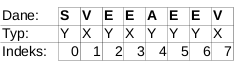
\includegraphics{\PICSDIR/bwt_dane}

\caption{\label{fig:Podzia=000142-danych-wej=00015Bciowych}Przykład - podział
danych wejściowych na typy}
\end{wrapfigure}%
%

\begin{figure}
\centering
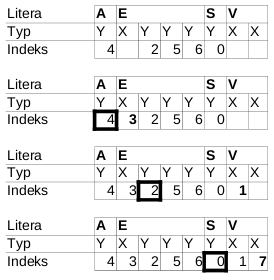
\includegraphics{\PICSDIR/bwt_dane3}

\caption{\label{fig:Spos=0000F3b-wstawiania-bajt=0000F3w}Przykład - sposób
wstawiania bajtów typu X do posortowanej tablicy. W pogrubionej ramce
znajduje się element powodujący wstawienie pogrubionego elementu typu
X.}

\end{figure}
Niewątpliwą zaletą zastosowanego algorytmu jest fakt, iż występujące
w kroku 3 łączenie koszyków ma złożoność liniową, co oznacza, że bajty
z koszyka X zostały posortowane w czasie liniowym. Pewną wadą przyjętego
rozwiązania jest to, iż w zależności od charakteru danych, spora ich
część trafia do koszyka Y, który jest już sortowany algorytmem Radix
Sort - podatnym na głęboką rekurencję.

Podczas dekodowania danych (transformata odwrotna - przywracająca
pierwotne ułożenie bajtów w bloku) stosowane jest sortowanie przez
zliczanie - ponieważ podczas dekodowania wystarczy posortować bajty
leksykograficznie (ściślej: tworzona jest tablica indeksów wskazujących
na posortowane dane). W związku z tym dekodowanie danych jest dużo
szybsze, niż kodowanie - algorytm sortowania przez zliczanie ma złożoność
liniową w stosunku do długości bloku. Pozostałe działania wykonywane
podczas dekodowania również posiadają liniową złożoność.

W transformacie bardzo ważny jest algorytm sortowania, ponieważ błędne
posortowanie danych powoduje przekłamania w odkodowanych danych.


\subsection{RLE0 i RLE2}
\label{ch:rle}
%% !TeX root = report.tex

W projekcie użyte zostały dwie odmiany algorytmu kodowania długości serii - RLE0 i RLE2. Podstawową różnicą w prezentowanych wersjach algorytmów jest sposób i miejsce zapisu informacji o długości znalezionego ciągu danych.

\subsubsection{RLE0}
RLE0\cite{deorowicz} jest najprostszą i najczęścej stosowaną implementacją tego algorytmu. Algorytm analizuje plik wejściowy znak po znaku i każdy ciąg znaków, zapisuje w postaci znaku reprezentującego ten ciąg i jego długości. Algorytm dzięki swej prostocie jest szybki, jednak w niesprzyjających warunkach prowadzi do wydłużenia danych zamiast ich kompresji.

\subsubsection{RLE2}
Podstawową różnicą pomiędzy RLE0 i RLE2\cite{abel} jest sposób przechowywania informacji o długości znalezionego ciągu. Algorytm analizuje dane wejściowe znak po znaku i w wypadku wykrycia ciągu o długości $n > 1$ zamienia taki ciąg na ciąg o długości dokładnie dwóch  znaków. Natomiast do drugiej tablicy zapisywana jet rzeczywista długość ciągu. Wykorzystanie RLE2 razem z algorytmem IFC (\ref{ch:ifc}) zostało opisane w \cite{abel}.

\subsection{Incremental Frequency Count}
\label{ch:ifc}
%% !TeX root = report.tex

Algorytm IFC (ang. Incremental Frequency Count) został stworzony i przez Jurgena Abela. Algorytm powstał by zaoferować skuteczną metodę przetwarzania danych otrzymanych z BWT. Założeniem było stworzenie algorytmu szybkiego i dającego dobre efekty kompresji. Algorytm został opisany w \cite{abel}. Daje on czasy działania porównywalne z MTF, przy jednoczesnym wysokim stopniu kompresji na poziomie algorytmu Sebastiana Deorowicza - WFC (ang. Weighted Frequency Count)\cite{deorowicz}.  

\begin{figure}
\centering
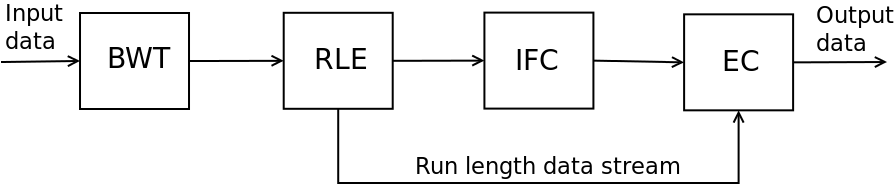
\includegraphics[width=\textwidth]{\PICSDIR/ifc}
\caption{Algorytm kompresji BWT z RLE2 i IFC}
\label{rys:bwca}
\end{figure}

Zadaniem algorytmu drugiej fazy kompresji BWT jest takie przetworzenie struktury z symboli otrzymanych z BWT by była ona łatwa do skompresowania przy użyciu kodeków entropijnych. W celu obliczania wartości wyjściowych w algorytmie IFC każdemu symbolowi przyporządkowywany jest licznik. Wszystkie licznik przechowywane są w kolejności malejącej. Dla każdego odczytanego z wejścia symbolu na wyjście wypisywana jest wartość licznika odpowiadającego temu symbolowi, po czym następuje przeliczenie wartości licznika. Podstawową ideą jest tutaj inkrementacja adaptacyjna bazująca na wykorzystaniu informacji o elementach które już się pojawiły. Liczniki poszczególnych elementów alfabetu mogą być inkrementowane lub dekrementowane w zależności od częstości występowania danego elementu. Powoduje to, że element występujące często mają niższe indeksy. Wartości liczników są co jakiś czas normowane. Główny nacisk kładziony jest w algorytmie na obliczanie wartości inkrementacji liczników. Algorytm podzielony jest na pięć części:
\begin{enumerate}
\item Wypisanie wartości odpowiedniego licznika na wyjście.
\item Obliczenie różnicy dla średniej wartości liczników dla poprzedniego i obecnego znaku. Wartości średnie obliczane są w przesuwnym oknie wg. wzoru:\\
$avg_{i} := \frac{(avg_{i-1} \dot (window\_size - 1)) - index_{x_{i}})}{windows\_size}$
\item Obliczenie wartości inkrementacji na podstawie różnicy średnich i wartości inkrementacji poprzedniego elementu:\\
$inc_i := inc_{i-1} - \frac{inc_{i-1} dif_i}{q}$, gdzie $q$ jest czynnikiem skalującym inkrementacji.
\item Przeskalowanie liczników jeżeli któryś z nich przekroczył wartość graniczną.
\item Ponowne posortowanie liczników. Sprowadza się to do odpowiedniego przesunięcia licznika elementu, który ostatnio pojawił się na wejściu. 
\end{enumerate}

\subsection{Distance Codding}
\label{ch:dc}
%% !TeX root = report.tex

Algorytm kodowania dystansowego (ang. Distance Coding - DC)\cite{deorowicz} został zaprezentowany w 2000 roku przez Edgara Bindera. Nie ma żadnej oficjalnej publikacji na jego temat. Został on zaproponowany na jednej z grup dyskusyjnych o kompresji danych. 

Dla każdego symbolu wejściowego $x_i^{bwt}$ algorytm znajduje odległość do jego następnego wystąpienia i ją zapisuje na wyjście. Jeżeli jest to ostanie wystąpienie elementu w ciągu wejściowym to na wyjście wypisywane jest $0$. Do poprawnego odczytania o ponownego zdekodowania zbioru wyjściowego niezbędna jest znajomość pozycji początkowych wszystkich elementów alfabetu występujących w analizowanym ciągu.

\subsection{Move To Front}
\label{ch:mtf}
%% !TeX root = report.tex

Move To Front (MTF) \cite{deorowicz} jest to prosta transformacja strumieniowa, której celem jest zmniejszenie entropii w kodowanym ciągu danych. Algorytm ten jest zalecany przez twórców BWT jako algorytm drugiego stopnia, najlepiej współpracujący z BWT. Algorytm operuje na danych wejściowych i liście $L$ zawierającej wszystkie elementy alfabetu. Początkowo lista $L$ jest posortowana w pewien ustalony sposób. Algorytm odczytuje z wejścia kolejne symbole ciągu wejściowego i dla każdego z nich na wyjście wyprowadzana jest pozycja odpowiadająca temu elementowi w liście $L$. Następnie lista jest modyfikowana tak, że element, który wystąpił jako ostatni wędruje na pierwszą pozycję. Taka modyfikacja powstanie ciągów powtarzających się elementów na wyjściu. Np. wszystkie ciągi jednakowych elementów zostaną zastąpione przez ciągi zer i jednej dodatkowej liczby stanowiącej pozycję początkową znaku. Do zdekodowania otrzymanego ciagu wyjściowego potrzebna jest jedynie wiedza na temat początkowego posortowania listy $L$ zawierającej alfabet.

\subsection{Invesrion Frequencies}
\label{ch:if}
%% !TeX root = report.tex

Algorytm IF (ang. Inversion Frequencies)\cite{deorowicz} został zaproponowany przez Arnavut i Magliveras w roku 1997. Jest on stosowany jako zamiennik MTF (\ref{ch:mtf}) w algorytmie kompresji BWT. Algorytm ten jako wyjście podaje sekwencje liczb z przedziału $[0; n -1]$, gdzie $n$ jest ilością elementów w ciągu wejściowym. Dla każdego elementu $a_i$ wykorzystywanego alfabetu algorytm skanuje sekwencje wejściową. W momencie pierwszego napotkania aktualnie analizowanego znaku $a_i$ algorytm wypisuje jego pozycję. Dla każdego kolejnego wystąpienia na wyjściu zapisywana jest liczba będąca ilością znaków większych niż analizowany element  $a_i$, która pojawiła się od jego ostatniego wystąpienia. Powstała w ten sposób sekwencja nie jest niestety wystarczająca do odkodowania danych wejściowych. Drugim niezbędnym elementem jest lista zawierająca ilość wystąpień każdego ze znaków w analizowanym ciągu.

\section{Testy}

\subsection{Aplikacja testująca}
\label{ch:app_test}
%% !TeX root = report.tex

W ramach projektu została stworzona aplikacja przeprowadzająca testy
algorytmu i wizualizująca wyniki kodowania. Jedną z jej części jest
program napisany w języku C++, odpowiedzialny za uruchomienie
właściwej aplikacji kodującej i pomiar czasu wykonania, którego wynik
przekazywany jest do aplikacji języka Java, pozwalającej na wybór
zestawu testów, parametrów algorytmów oraz prezentację i porównanie
wydajności algorytmów. Wybór możliwy jest spośród 9 wariantów pracy
stworzonego w ramach projektu kodera oraz algorytmu Bzip2 w
standardowej implementacji dla systemu Linux. Dodatkowo dla naszego
kodera istnieje możliwość ustawienia parametru --- rozmiaru bloku BWT ---
od 1 do 8192 kB.

Główne okno aplikacji składa się z trzech części --- w lewym górnym
rogu znajdują się zakładki sterujące pracą aplikacji, w prawym górnym
roku widoczna jest konsola tekstowa, a w dolnej części prezentowane są
wykresy średniej bitowej oraz czasu kodowania kolejnych plików
testowych dla wybranych algorytmów.

Zakładka {\em Plik} pozwala na przeprowadzenie pojedynczego testu. 3
przyciski pozwalają na wybór pliku, przeprowadzenie kompresji i
dekompresji. Możliwy jest również wybór algorytmu i rozmiaru bloku
BWT. Dodatkowo dla pliku przed kompresją, po kompresji oraz po
dekompresji prezentowana jest nazwa, rozmiar oraz wyliczona suma
CRC32, dzięki czemu można szybko stwierdzić, czy operacje zostały
przeprowadzone prawidłowo. Po przeprowadzeniu kompresji jej czas i
uzyskana średnia bitowa nanoszona jest na wykres. Informacje te można
także przeczytać z konsoli.

Zakładka {\em Zestaw} pozwala na przeprowadzenie testu 3 wybranych
algorytmów na podstawie plików zawartych w jednym z czterech zbiorów
testowych. Dla każdego algorytmu istnieje możliwość indywidualnego
ustawienia rozmiaru bloku BWT. W czasie przeprowadzania testu wykres
oraz informacje na konsoli uaktualniane są na bieżąco. Po zakończeniu
wszystkich operacji generowana jest tabela zawierająca zestawienie
wyników i wyliczenie średnich poszczególnych algorytmów dla wszystkich
plików. Jeśli opcja Dekompresja zostanie zaznaczona przeprowadzona
zostanie także procedura dekompresji i czasy jej wykonania zostaną
zebrane w tabeli.

Na wykresie trzema kolorami przedstawione są rezultaty poszczególnych
algorytmów. Wysokość słupka wyraża względną średnią bitową, natomiast
wartości czasu kompresji łączone są linią tworząc wykres liniowy na
każdego algorytmu z osobna. Dodatkowo pod słupkiem znajduje się
informacja o nazwie kompresowanego pliku, wybranym algorytmie oraz
rozmiarze bloku BWT.

\begin{figure}[htb]
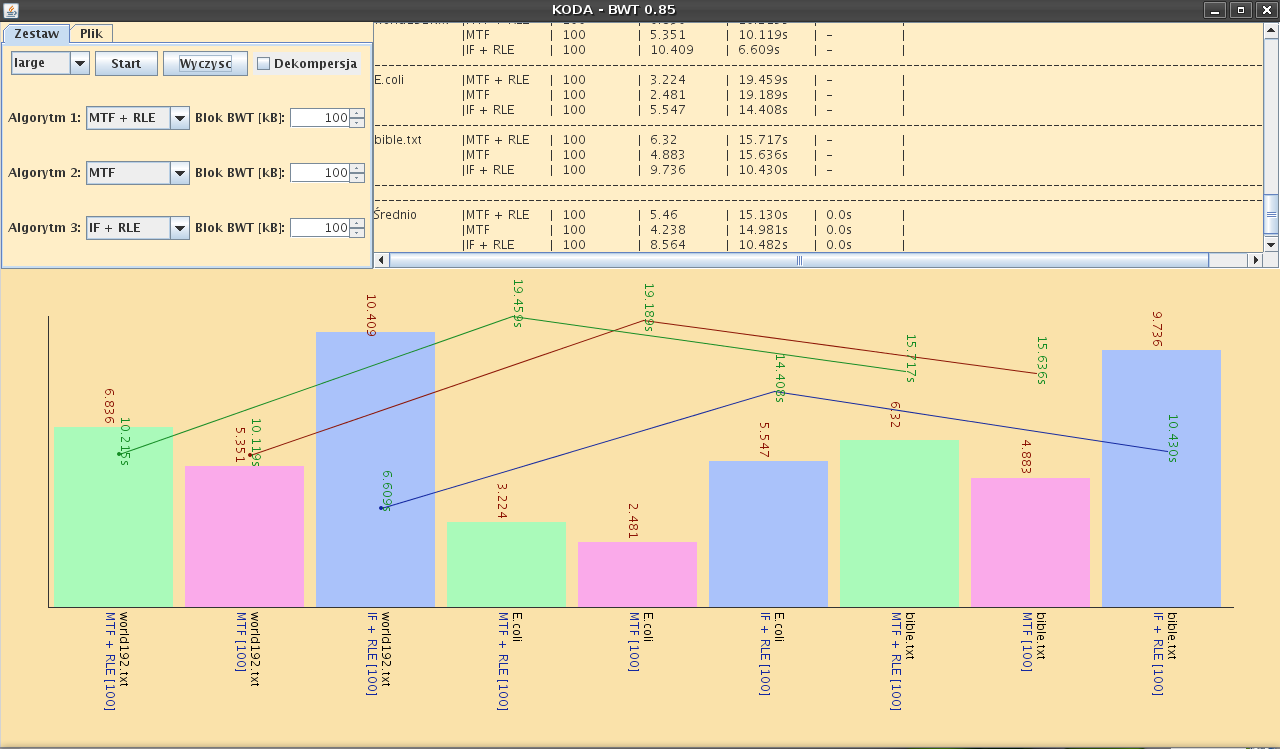
\includegraphics[scale=0.35]{\PICSDIR/test.png}
\caption{\label{fig:aplikacja_testujaca}Ekran główny aplikacji testującej}
\end{figure}

\subsection{Testy wydajności}

\subsubsection{Dane testowe}
%% !TeX root = report.tex
%% 
Zbiór {\em artificl} zawiera cztery sztucznie wygenerowane pliki
zawierające odpowiednio: jedną literę a {\em (a.txt)}, powtarzające się
litery a {\em (aaa.txt)}, powtarzający się alfabet {\em (alphabet.txt)} oraz
litery w kolejności pseudolosowej {\em (random.txt)}. Może być on pomocny w
sprawdzeniu jak algorytmy zachowują się w najgorszym możliwym
scenariuszu (losowe znaki, bardzo mały plik).

Zbiór {\em calgary} zawiera 18 plików różnego typu stanowiących {\em The Calgary
Corpus}, standard dla badania wydajności bezstratnej kompresji w latach
90. ubiegłego wieku.

Zbiór {\em cantrbry} zawiera 11 plików stanowiących {\em The Canterbury Corpus}.
Jest to zbiór utworzony w 1997 roku jako udoskonalenie poprzedniego
zbioru. Pliki zostały tak dobrane, że ich rezultat przy wykorzystaniu
ówczesnych algorytmów kompresji był reprezentatywny i stąd nadzieja, że
będzie on taki także dla nowych metod kompresji.

Zbiór {\em large} zawiera 3 duże pliki (od 2 do 4,4 MB każdy) --- kompletny
genom bakterii E. Coli, jedna z wersji Biblii oraz opis krajów świata
--- {\em The CIA world fact book}.

\subsubsection{Wyniki}
%% !TeX root = report.tex

\paragraph{Zbiór large}

Pierwszym przeprowadzonym testem był test wszystkich wersji algorytmu dla zbioru {\em large}. Rozmiar bloku BWT ustawiony został na wartość równą 4 MB, czyli nieco mniejszą niż rozmiar największego pliku.

\begin{figure}[phtb]
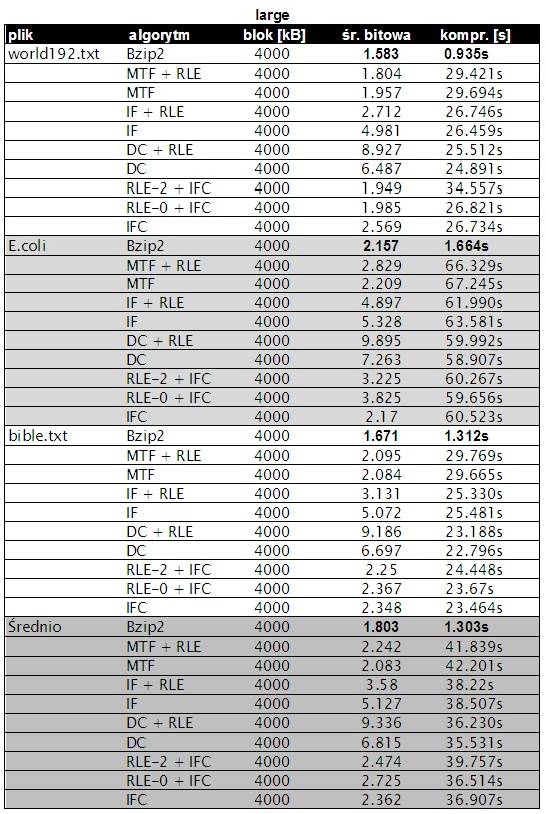
\includegraphics[scale=1.0]{\PICSDIR/tab_large_wszystkie.jpg}
\caption{\label{fig:tab_large_wszystkie}Wyniki testu dla zbioru large}
\end{figure}

Dla tych plików najlepszym okazał się referencyjny algorytm Bzip2, jednak pod względem wartości średniej bitowej niewiele gorszy okazał się algorytm MTF. Różnica wynosi jedynie 15 proc. Następne miejsce zajął algorytm MTF+RLE, a kolejne algorytmy wykorzystujące IFC. Dużo gorzej wypadły metody IF i DC.
 
Niestety pod względem czasu trwania kompresji nasz algorytm znacznie odbiegał od Bzip2. Najdłużej działała metoda, która uzyskała najlepszy wynik pod względem wartości średniej bitowej (MTF) i czas ten był aż 32 razy dłuższy od referencyjnego Bzip2.

\paragraph{Badanie wpływu rozmiaru bloku BWT}

\begin{figure}[phtb]
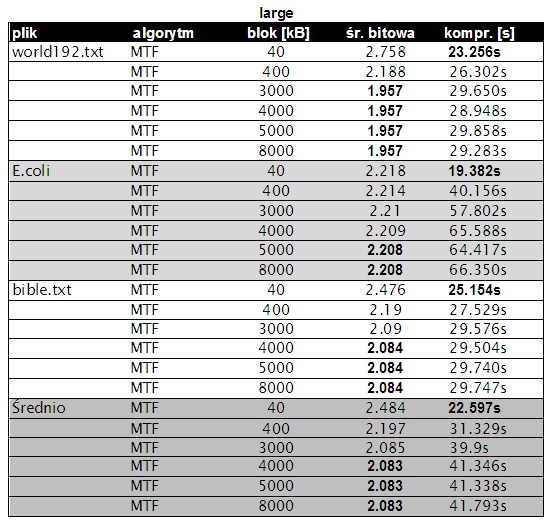
\includegraphics[scale=1.0]{\PICSDIR/tab_large_badanieBlokSize.jpg}
\caption{\label{fig:tab_large_badanieBlokSize}Wyniki testu parametru rozmiaru bloku BWT dla zbioru large}
\end{figure}

Algorytm, który uzyskał najlepszą średnią bitową w poprzednim teście posłużył do wykonania testu wpływu wartości parametru rozmiaru bloku BWT na jakość kompresji. Zgodnie z przewidywaniami, im większa wartość bloku tym algorytm BWT lepiej radzi sobie z kompresją, ale wzrasta długość trwania kompresji. Ograniczeniem jest długość samego pliku poddawanego poszczególnym operacjom. W dalszych testach wartość tego parametru pozostała na poziomie 4 MB, gdyż tylko rozmiar jednego z testowanych plików przekracza tą wartość, a dalszy wzrost tego parametru poprawia średnią bitową dla tego pliku o mniej niż jeden promil.

\paragraph{Zbiór canterbry}

\begin{figure}[phtb]
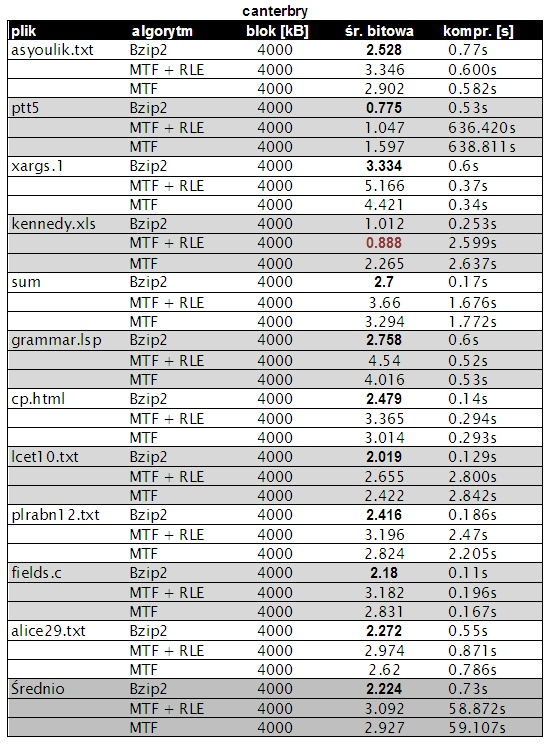
\includegraphics[scale=1.0]{\PICSDIR/tab_canterbry_lepszyNizBzip2.jpg}
\caption{\label{fig:tab_canterbry_lepszyNizBzip2.jpg}Wyniki testu dla zbioru canterbry}
\end{figure}

Po przeprowadzeniu testów na zbiorze {\em canterbry} dla 3 najlepszych algorytmów okazało się, że dla niektórych plików jeden z wariantów naszego algorytmu (MTF+RLE) może uzyskiwać mniejszą średnią bitową niż referencyjny Bzip2. Stało się tak dla pliku arkusza kalkulacyjnego {\em kennedy.xls}. Dodatkowo dla kilku innych plików uzyskaliśmy krótszy czas kompresji ({\em asyoulik.txt, xargs.1, grammar.lsp}). 

Niestety, nasz algorytm dla niektórych plików uzyskuje czas kompresji rzędu kilku minut, mimo że nie są to duże pliki. Związane jest to z algorytmem sortowania użytym w BWT.

\paragraph{Zbiór calgaryS}

Po usunięciu ze zbioru calgary pliku {\em pic}, dla którego czas kompresji wynosił 10 minut, powstał zbiór {\em calgaryS}, dla którego przeprowadziliśmy testy wszystkich algorytmów. Średnie wyniki zostały zebrane w poniższej tabeli. Zamieszczone zostały także wykresy wartości średniej bitowej i czasu kompresji. Kolejność pod względem wartości średniej bitowej odpowiada kolejności dla zbioru {\em large}. W tym teście zostały dodatkowo zbadane czasy trwania dekompresji. Jedynie dla algorytmu RLE-2 + IFC czas dekompresji dwóch plików wyniósł 30 sekund, co spowodowało znaczący wzrost średniej. Pozostałym algorytmom dekompresja zajmowała najczęściej mniej niż jedną sekundę.

\begin{figure}[phtb]
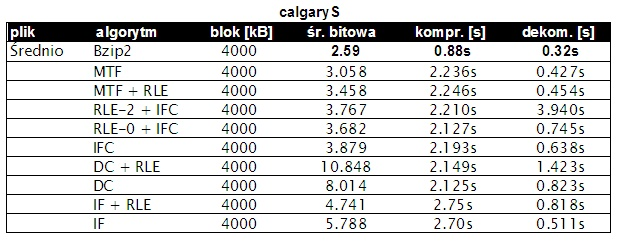
\includegraphics[scale=1.0]{\PICSDIR/tab_calgaryS_wszystkie.jpg}
\caption{\label{fig:tab_calgaryS_wszystkie.jpg}Wyniki testu dla zbioru calgaryS}
\end{figure}

\begin{figure}[phtb]
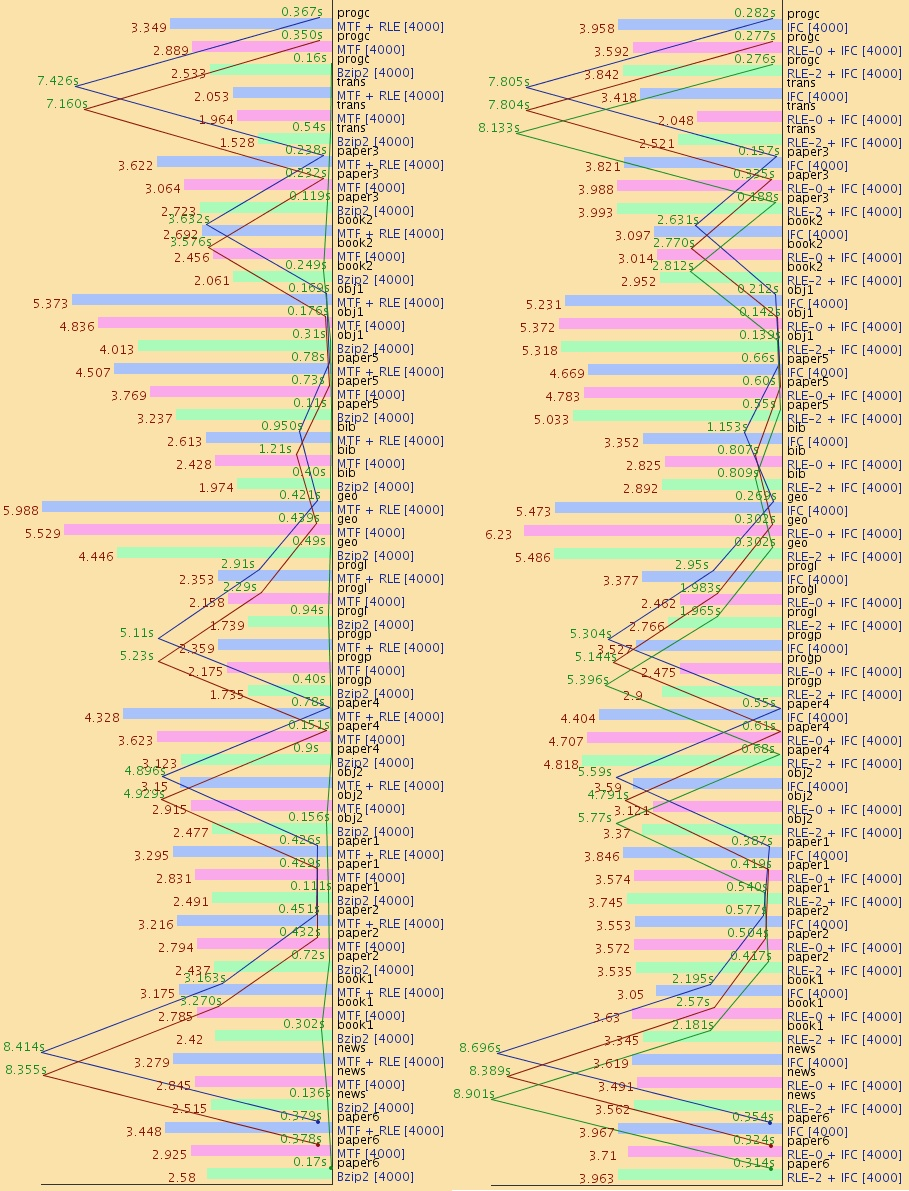
\includegraphics[scale=0.7]{\PICSDIR/graph_calgaryS_Bzip2_MTF_IFC.jpg}
\caption{\label{fig:graph_calgaryS_Bzip2_MTF_IFC.jpg}Wyniki testu dla zbioru calgaryS, algorytmy MTF i IFC}
\end{figure}

\begin{figure}[phtb]
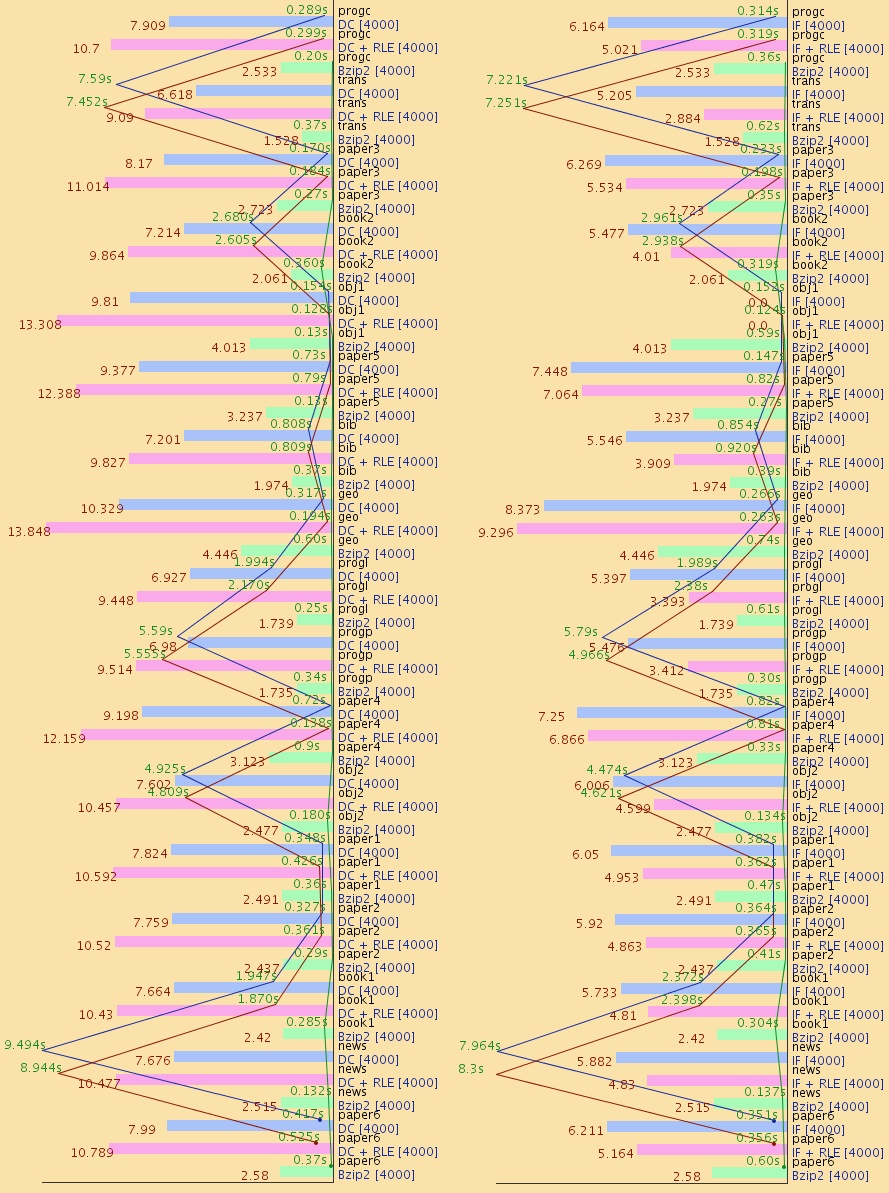
\includegraphics[scale=0.7]{\PICSDIR/graph_calgaryS_Bzip2_DC_IF.jpg}
\caption{\label{fig:graph_calgaryS_Bzip2_DC_IF.jpgg}Wyniki testu dla zbioru calgaryS, algorytmy DC i IF}
\end{figure}

\paragraph{Zbiór artificl}

Przeprowadzony został także test dla zbioru plików sztucznych. Algorytm MTF uzyskał najlepsze czasy kompresji dla pliku zawierającego pojedynczą literę ({\em a.txt}) oraz znaki w losowej kolejności ({\em random.txt}). Czasy te były lepsze także od czasów referencyjnego algorytmu Bzip2. Jednakże kompresja pozostałych dwóch plików zajęła kilka minut, a  średnie bitowe były gorsze.

\begin{figure}[phtb]
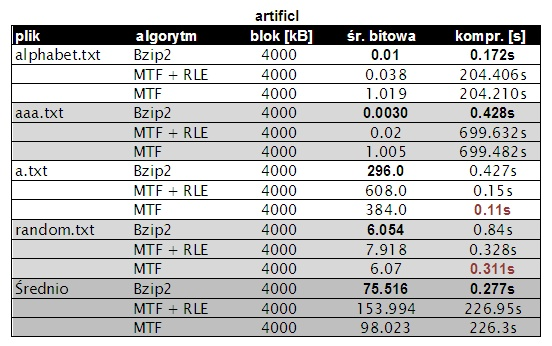
\includegraphics[scale=1.0]{\PICSDIR/tab_artificl_mtfrle.jpg}
\caption{\label{fig:tab_artificl_mtfrle.jpg}Wyniki testu dla zbioru artificl}
\end{figure}


%% !TeX root = report.tex

\section{Napotkane trudności}

W czasie tworzenia przedstawionej w tym raporcie prezentacji napotkane zostały pewne trudności. Przede wszystkim najpoważniejszą było podejście do takiego implementowania algorytmów, by wynikowe, skompresowane dane zajmowały jak najmniej miejsca. Podstawowym problemem w przypadku takich algorytmów jak Distance Coding, Inversion Frequencies czy Huffman Coding był problem zapisu dodatkowych informacji niezbędnych przy dekompresji. Każdy z wymienionych algorytmów do poprawnego działania potrzebuje dodatkowych danych np. w algorytmie IF niezbędna jest lista zawierająca liczbę wystąpień każdego znaku. Takie dodatkowe dane stanowią szczególny problem w wypadku małych plików, gdyż ich długość, która musi być dodana do pliku wynikowego może nawet kilkukrotnie przekraczać długość skompresowanych danych.

\section{Podsumowanie}

W ramach projektu stworzona została implementacja algorytmów kompresji BWT. Zaimplementowane zostały oprócz samej transformaty różnego rodzaju algorytmy drugiego kroku. Algorytmy te są dość zróżnicowane pod względem czasu działania, uzyskiwanych wyników kompresji, prostoty implementacji.

Stworzona implementacja okazała się być (WYDAJNA?/ NIE?) co pokazują wyniki przeprowadzonych testów.

Co ciekawego udało nam się zrobić?
	- uzyskać lepszą średnią bitową niż Bzip2 dla jednego pliku
	- uzyskać lepsze czasy kompresji dla kilku plików
	- sprawdzić nowe algorytmy fazy drugiej (IFC)


\clearpage

\bibliography{mybib}{}
\bibliographystyle{plain}

\end{document}
